% The Potts factor graph of Section~\ref{sec:potts}, drawn by hand. Input by
% textbook.tex; a sketch and not a rendered figure, so it is outside the
% figure cache and the render cap, which govern generated output only.
\begin{figure}[htbp]
\centering
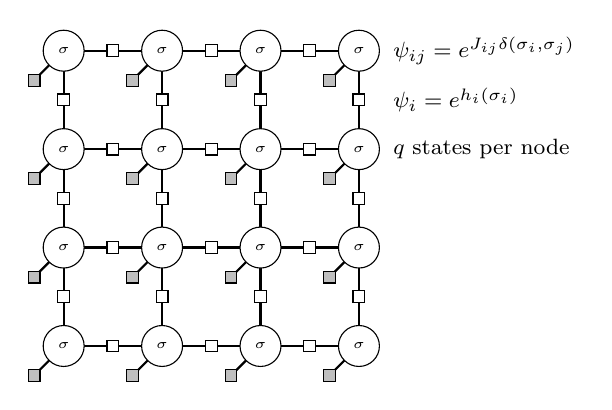
\begin{tikzpicture}[
    scale=1.25,
    spin/.style={circle, draw, minimum size=0.52cm, inner sep=0pt, font=\tiny, fill=white},
    factor/.style={rectangle, draw, fill=white, minimum size=0.15cm, inner sep=0pt},
    field/.style={rectangle, draw, fill=black!25, minimum size=0.15cm, inner sep=0pt},
    bond/.style={draw, thick}
]
  % Pairwise factors, one per edge of the open square lattice.
  \foreach \i in {0,...,3} {
    \foreach \j in {0,...,3} {
      \ifnum\i<3
        \draw[bond] (\i, \j) -- (\i+1, \j);
        \node[factor] at (\i+0.5, \j) {};
      \fi
      \ifnum\j<3
        \draw[bond] (\i, \j) -- (\i, \j+1);
        \node[factor] at (\i, \j+0.5) {};
      \fi
    }
  }
  % One field factor per node, on a stub so it is not mistaken for a bond.
  \foreach \i in {0,...,3} {
    \foreach \j in {0,...,3} {
      \draw[bond] (\i, \j) -- (\i-0.30, \j-0.30);
      \node[field] at (\i-0.30, \j-0.30) {};
      \node[spin] at (\i, \j) {$\sigma$};
    }
  }
  \node[anchor=west, font=\footnotesize] at (3.25, 3.0)
    {$\psi_{ij} = e^{J_{ij}\delta(\sigma_i,\sigma_j)}$};
  \node[anchor=west, font=\footnotesize] at (3.25, 2.5)
    {$\psi_{i} = e^{h_i(\sigma_i)}$};
  \node[anchor=west, font=\footnotesize] at (3.25, 2.0)
    {$q$ states per node};
\end{tikzpicture}
\caption{A Potts model in an external field as a factor graph, on the open
$4 \times 4$ square lattice. Circles are the spins $\sigma_i \in \{1, \dots,
q\}$; open squares on each edge are the pairwise factors of
Equation~\ref{eq:potts} and shaded squares on a stub are the unary field
factors. The graph has cycles, so Equation~\ref{eq:sum-product} on it is the
Bethe approximation of Equation~\ref{eq:bethe} and not the exact marginal;
the square lattice is two-colourable, so it also carries no frustration,
which is what Section~\ref{sec:frustrated} adds. A sketch of the structure
and not a rendering of any instance.}
\label{fig:potts:sketch}
\end{figure}
